\section{Hệ mật trên đường cong Elliptic}

\subsection{Đường cong Elliptic}

Đường cong Elliptic trong hệ toạ độ $Oxy$ có công thức tổng quát như sau:
$$
y^2\pmod{p}\equiv x^3+ax+b\pmod{p},
$$
trong đó $a$, $b$ là các tham số thực, $p$ là một số nguyên dương ngẫu nhiên.\\

\begin{figure}[!ht]
    \centering
    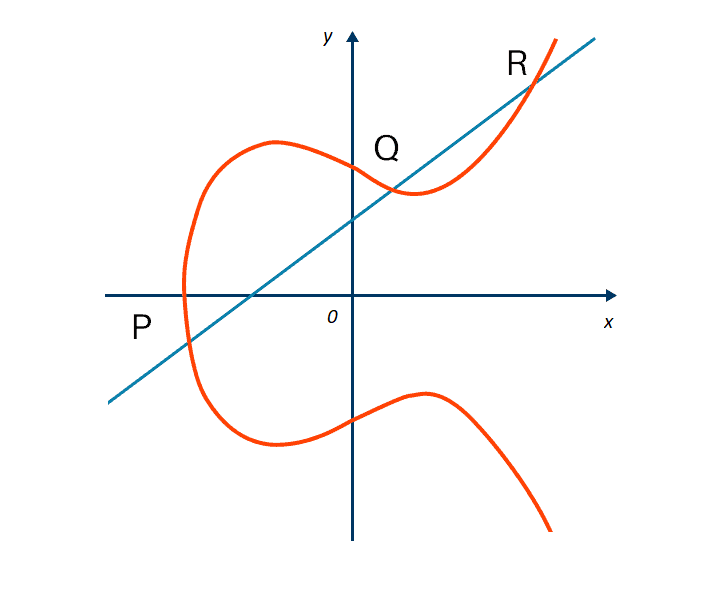
\includegraphics[width=400px]{anh/mat-ma-hoa-khoa-cong-khai/ecc.png}
    \caption{Hình dạng của đường cong Elliptic trên hệ trục toạ độ $Oxy$.}
\end{figure}

Viện Tiêu chuẩn và Kỹ thuật Quốc gia Mỹ (NIST) đặt ra tiêu chuẩn \textit{secp256k1} với công thức của đường cong Elliptic như sau:
$$
y^2\pmod{p}\equiv x^3+7\pmod{p},
$$
với $p$ là một số nguyên tố rất lớn:
$$
p=2^{265}-2^{32}-2^9-2^8-2^7-2^6-2^4-1.
$$

\subsection{Các phép toán trên đường cong Elliptic}

Có hai phép toán quan trọng trên đường cong Elliptic: Phép cộng và phép nhân.

\subsubsection*{Phép cộng}

Đường cong Elliptic có một tính chất: "Nếu hai điểm $P$ và $Q$ nằm trên đường cong, thì điểm $P+Q$ cũng nằm trên đường cong đó.".\\

Điểm $P+Q$ được xác định như sau:
\begin{itemize}
    \item Vẽ đường thẳng nối hai điểm $P$ và $Q$, đường thẳng này cắt đường cong tại một điểm nữa, gọi là $R$.
    \item Lấy đối xứng của điểm $R$ đó qua trục hoành, ta được điểm $P+Q$.
\end{itemize}

Và từ đó, ta có tính chất sau: "Nếu ba điểm trên đường cong Elliptic thẳng hàng, tổng của chúng bằng $0$".

\subsubsection*{Phép nhân}

Trên đường cong Elliptic, việc nhân một điểm với một hằng số không đơn thuần chỉ là lấy từng toạ độ rồi nhân là xong. Thực chất, phép nhân ở đây được thực hiện bằng cách lặp lại nhiều lần phép cộng.\\

Ví dụ trong phép tính $3P$, đầu tiên ta tính $2P$ bằng cách thực hiện $P+P$. Theo cách cộng ở bên trên, ta vẽ đường thẳng nối $P$ với $P$ (chính là tiếp tuyến của đường cong), nó cắt đường cong tại điểm $-2P$. Lấy đối xứng qua trục hoành, ta có điểm $2P$. Tiếp tục vẽ đường thẳng nối giữa $2P$ và $P$, cắt đường cong tại $-3P$, lấy đối xứng ta có $3P$.\\

Do cách tính toán trên, ta có thể dễ dàng tính toán được phép nhân $kP$ khi biết $k$ và $P$, nhưng hoàn toàn không thể tính toán được theo chiều ngược lại, tức phép chia. Đó cũng chính là tính chất đặc trưng thú vị của mã hoá bất đối xứng.

\subsection{Tạo khoá công khai}

Giả sử ta đã có khoá bí mật là một số ngẫu nhiên $d_A$. Trên đường cong Elliptic, ta chọn một điểm $G$, gọi là điểm sinh (generator point hay reference point).\\

Khoá công khai $Q_A$ được sinh ra bằng kết quả của phép nhân:
$$
Q_A=d_A\times G.
$$

Tất nhiên $Q_A$ cũng là một điểm trên đường cong Elliptic. Mối quan hệ giữa $d_A$ và $Q_A$ là cố định, và chỉ tính được theo một chiều từ $d_A$ đến $Q_A$. Đó là lý do tại sao ta có thể sinh ra khoá công khai từ khoá bí mật và có thể chia sẻ khoá công khai này với tất cả mọi người, mà không thể dùng khoá công khai để tìm ngược lại về khoá bí mật.